\documentclass[runningheads]{llncs}

\usepackage[T1]{fontenc}
\usepackage{graphicx}
\usepackage{amsmath}
\usepackage{amssymb}
\usepackage{booktabs}
\usepackage{multirow}
\usepackage{tabularx}
\usepackage{float}
\usepackage{tikz}
\usetikzlibrary{arrows.meta,calc,fit,matrix,positioning}
\usepackage{url}
\emergencystretch=2em

\newcommand{\R}{\mathbb{R}}
\newcommand{\Lbase}{\mathcal{L}_{\mathrm{base}}}
\newcommand{\Lglobal}{\mathcal{L}_{\mathrm{gSC}}}
\newcommand{\Lpart}{\mathcal{L}_{\mathrm{pSC}}}
\newcommand{\Lptrip}{\mathcal{L}_{\mathrm{pTri}}}

\begin{document}

\title{Training Parts vs. Matching Parts: A Controlled Study of Part-Level Objectives for Occlusion-Robust Pose Gait Recognition}
\titlerunning{Training Parts vs. Matching Parts for Pose Gait Recognition}

\author{Minas Aslanyan\inst{1} \and Levon Aslanyan\inst{1}}
\authorrunning{M. Aslanyan and L. Aslanyan}

\institute{Institute for Informatics and Automation Problems, National Academy of
Sciences of the Republic of Armenia (IIAP), Yerevan, Armenia\\
\email{minas.aslanyan@gmail.com, lasl@sci.am}}

\maketitle

\begin{abstract}
Part-level learning is a plausible response to occluded gait: if one limb is
missing, the remaining anatomical regions should still support retrieval.
However, it is unclear whether parts should be supervised during training,
used only during matching, or reliability-gated in both stages. We conduct a
controlled development and official-test study on 2D pose sequences from
CASIA-B. On a 12-identity development split, a common multistream graph
backbone is trained under six objectives using three seeds. The metric baseline
is strongest: adding part supervised contrastive learning reduces averaged
corrupted-probe Rank-1 from 63.90\% to 57.78\%, a paired difference of $-6.12$
percentage points with a hierarchical 95\% bootstrap interval of
$[-9.54,-2.68]$. Freezing the baseline checkpoints and replacing the untrained
local projections with normalized pre-projection part pools raises the same
endpoint to 68.23\%, a gain of $+4.32$ points, $[+3.25,+5.35]$. We then retrain
the metric baseline on all 74 official training identities with five seeds and
evaluate the untouched 50-identity test split. Under the standard single-view
CASIA-B protocol, global matching obtains $48.35\pm1.85$\% average Rank-1,
whereas reliability-weighted raw-part matching obtains $54.04\pm2.18$\%.
The paired gain is $+5.69$ points with a 95\% interval of
$[+5.19,+6.20]$. Pooled multi-view test outcomes and synthetic corruptions also
favor raw-part matching, with gains of $+6.58$, $+6.39$, and $+5.63$ points for
uncorrupted, corrupted-probe, and independently corrupted-gallery endpoints.
Uniform raw-part averaging reaches the same 54.04\% standard-protocol average,
so reliability gating is not a material independent contribution. The evidence
rejects the tested part-level training objectives while supporting a simpler
conclusion: match anatomical features already present in the globally trained
backbone without learning a local projection. Real-occlusion and external-
dataset confirmation remain necessary.

\keywords{gait recognition \and 2D pose \and occlusion robustness \and
supervised contrastive learning \and part-based matching \and negative results}
\end{abstract}

\section{Introduction}

Gait recognition supports identity retrieval at a distance, including cases in
which face evidence is weak or unavailable. Pose-based methods replace raw
appearance with joint trajectories and can reduce dependence on clothing,
background, and illumination \cite{liao2020posegait}. Graph encoders such as
ST-GCN \cite{yan2018stgcn}, GaitGraph \cite{teepe2021gaitgraph}, and GaitGraph2
\cite{teepe2022gaitgraph2} make this representation computationally natural.
Its main weakness is equally direct: a pose sequence
contains only the body evidence recovered by the pose estimator. Occlusion,
truncation, detector uncertainty, and identity overlap can remove joints or
produce anatomically inconsistent tracks. Recent surveys and dedicated
occluded-gait benchmarks consequently identify partial body evidence as a
central challenge \cite{li2024survey,huang2024occluded}.

An intuitive remedy is to learn anatomical embeddings. Supervised contrastive
learning can align two corrupted observations of the same identity while
separating different identities \cite{khosla2020supervised}. A part-level
extension can apply the same objective independently to the torso and four
limbs, weighting each term by the observed pose confidence. This argument is
plausible, but it combines three decisions that need not have the same answer:
whether to train local heads, whether to gate their training loss, and whether
to use local scores during retrieval. A method can benefit from part-aware
matching even when an auxiliary part loss conflicts with the primary identity
objective. Conversely, a trained local head can collapse or overfit synthetic
missingness.

This paper separates these decisions in a controlled factorial development
study followed by a fixed official-test confirmation. Every
configuration uses the same 2D input, augmentation distribution, multistream
graph backbone, batch construction, clean classification anchor, global
batch-hard triplet loss, checkpoint-selection rule, and evaluation masks. Only
the auxiliary global or part metric term changes. Each configuration is trained
with seeds 11, 22, and 33 on the development split. After selecting the raw-part
matcher, we retrain only the metric baseline on all 74 official training
identities using seeds 11, 22, 33, 44, and 55 and evaluate identities 075--124.
Saved probe-level correctness outcomes permit paired resampling over identities
rather than treating aggregate accuracy cells as independent observations.

The study asks five questions:
\begin{enumerate}
    \item Does global supervised contrastive learning improve a strong
    classification-plus-triplet baseline?
    \item Does part-level supervised contrastive learning improve robustness,
    and does reliability gating explain its effect?
    \item Does a part-level triplet objective provide a better-trained local
    descriptor than part supervised contrastive learning?
    \item Is part-aware matching useful independently of part-aware training?
    \item Does the selected matcher carry over to the official CASIA-B test
    identities without further tuning?
\end{enumerate}

The observed answers are negative for auxiliary part training and positive for
local matching. Global SupCon is statistically inconclusive relative to the
baseline. Part SupCon produces a clear robustness loss. Ungating recovers only
part of the deficit. Part triplet collapses its local embedding variance and
does not improve retrieval. In contrast, deterministic matching of normalized
pre-projection part pools improves clean and corrupted recognition for every
training seed and all four corruption families. Ten freshly initialized frozen
heads confirm that the earlier gain is not dependent on one favorable random
projection; nevertheless, the raw descriptor is stronger and removes the
projection entirely. The official-test experiment preserves this conclusion:
both raw-part variants improve NM, BG, and CL recognition over global matching,
while reliability-weighted and uniform part averaging remain effectively tied.

The contribution is therefore not a state-of-the-art accuracy claim. It is an
auditable diagnosis of a common design assumption, supported by a complete
$6\times3$ run matrix, checkpoint-only controls spanning ten random projections
and five fusion weights, paired probe outcomes, and training diagnostics. A
separate five-seed official-test experiment confirms the selected
parameter-free descriptor under the standard CASIA-B protocol and controlled
synthetic corruptions. The results illustrate why clean accuracy alone is
insufficient for selecting an occlusion-robust gait objective.

\section{Related Work}

\subsection{Contrastive learning for structured motion}

SimCLR and MoCo established the importance of positive-pair construction,
projection heads, and negative sampling in visual contrastive learning
\cite{chen2020simclr,he2020moco}. Supervised contrastive learning extends the
positive set to all same-class observations \cite{khosla2020supervised}. For
skeleton sequences, domain-specific transformations are required because an
arbitrary image augmentation need not preserve joint semantics. Skeleton-
Contrastive learning uses multiple skeleton representations and motion-aware
transformations for action recognition \cite{thoker2021skeleton}; prototype
contrastive learning has also been applied to skeleton person
re-identification \cite{rao2024skeleton}. More recently, GaitPT studied model,
data, and compute scaling for self-supervised skeleton gait pretraining on
millions of in-the-wild sequences \cite{cosma2026gaitpt}. These results motivate
contrastive objectives, but they do not establish that independent anatomical
objectives help fine-grained gait identity retrieval.

\subsection{Pose-based gait and occlusion}

PoseGait established a compact 3D-pose route to model-based recognition
\cite{liao2020posegait}. GaitGraph and GaitGraph2 subsequently demonstrated
graph convolution with learned spatial--temporal and multistream skeleton
features \cite{teepe2021gaitgraph,teepe2022gaitgraph2}. GPGait adds
human-oriented normalization and a part-aware graph network for cross-dataset
generalization \cite{fu2023gpgait}, while SkeletonGait converts joints to
heatmap-like skeleton maps to recover structural cues that coordinate-only
models may underuse \cite{fan2024skeletongait}. OpenGait emphasizes standardized
protocols and reproducible evaluation across gait datasets
\cite{fan2022opengait}.

Occlusion is heterogeneous: random joint loss, a missing limb, a continuous
temporal interruption, and a real detector failure produce different evidence
distributions \cite{li2024survey}. OccGait and GaitMoE further show that real
occlusion combines missing information with misalignment and noise
\cite{huang2024occluded}. Related skeleton work has combined partial
spatio-temporal learning with imputation in occluded action recognition
\cite{chen2023iopstl}. Large in-the-wild benchmarks such as GREW and Gait3D
also expose shifts and nuisance factors absent from controlled laboratory data
\cite{zhu2021grew,zheng2022gait3d}. Our study does not claim that synthetic
masks substitute for these real errors. Instead, it uses deterministic
synthetic families to isolate objective and matching effects before external
validation.

\subsection{Part-aware gait representation}

Part modeling is well established in appearance-based gait recognition.
GaitPart assigns separate short-range temporal models to horizontal body
regions \cite{fan2020gaitpart}; GaitGL couples global and local feature
extraction \cite{lin2021gaitgl}; and 3D Local CNNs learn part-specific
spatio-temporal neighborhoods \cite{huang2021local}. GPGait is more directly
related to our pose setting because its graph partition explicitly captures
local--global keypoint relations \cite{fu2023gpgait}. These works support the
value of anatomical structure, but they jointly change representation,
architecture, and training. They therefore do not answer the narrower question
studied here: with a fixed pose backbone, should local parts receive their own
metric objective, enter the matcher, or both?

\subsection{Position of this study}

Most method papers compare a complete proposal with a small set of baselines.
Here the main object is the interaction between training objective and retrieval
descriptor. All methods share the same backbone and occlusion exposure. We
explicitly retain results that contradict the original hypothesis and use
run-level artifacts to distinguish three possible explanations: ineffective
global contrast, harmful local supervision, and descriptor-head behavior.

\section{Controlled Study}

Figure~\ref{fig:framework} summarizes the controlled design. Training changes
only the auxiliary objective attached to shared global or anatomical features;
the checkpoint-only control study freezes the baseline encoder and changes only
the local descriptor and matching rule.

\begin{figure}[t]
\centering
\resizebox{\textwidth}{!}{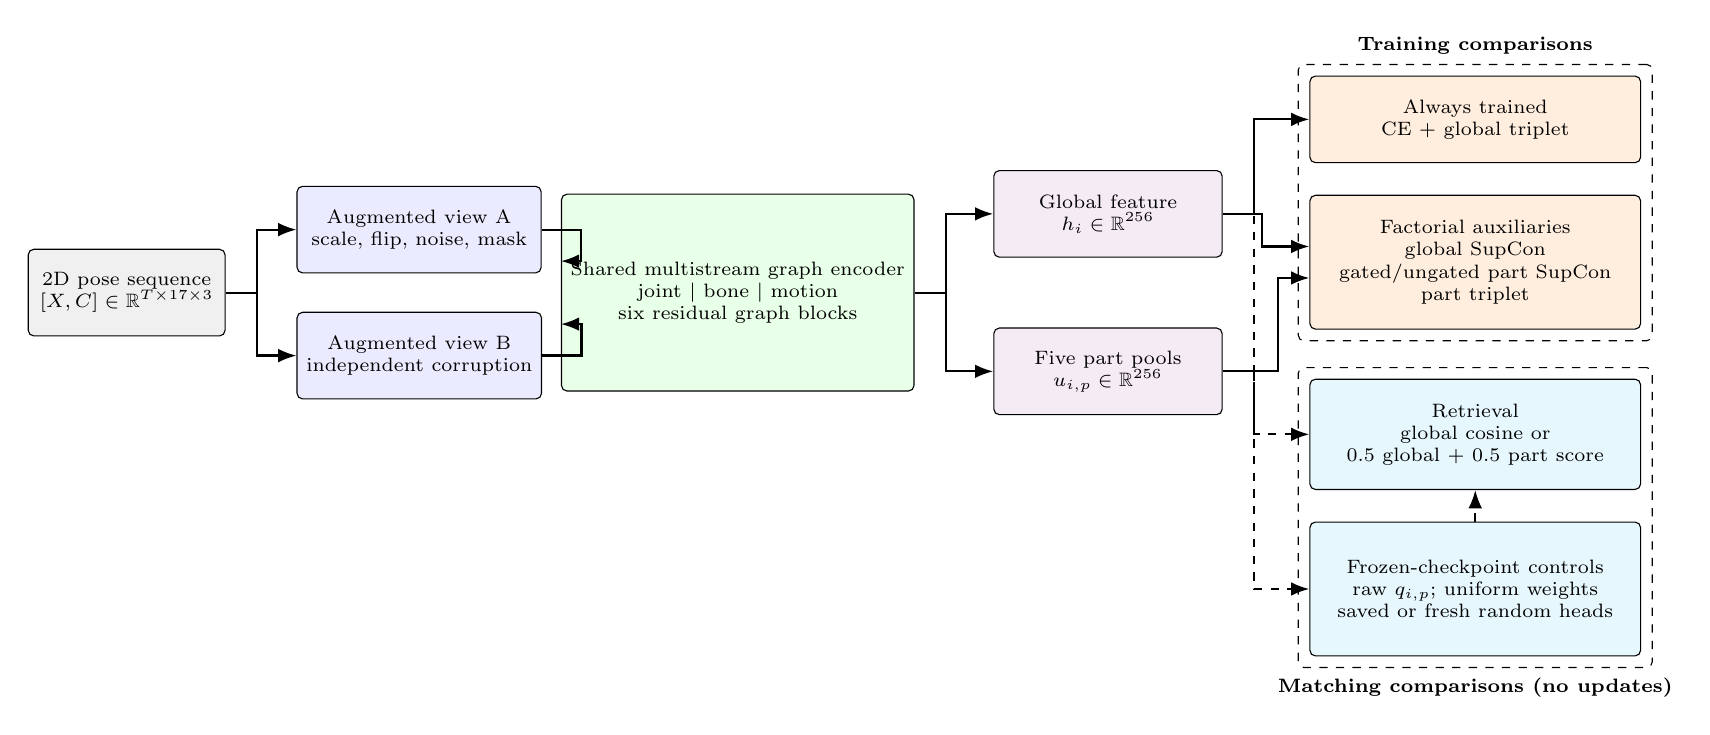
\begin{tikzpicture}[
    font=\scriptsize,
    box/.style={draw, rounded corners=2pt, align=center, minimum width=25mm,
        minimum height=11mm, fill=gray!8},
    view/.style={box, fill=blue!8, minimum width=31mm},
    encoder/.style={box, fill=green!9, minimum width=38mm, minimum height=25mm},
    feature/.style={box, fill=violet!8, minimum width=29mm},
    train/.style={box, fill=orange!13, minimum width=42mm},
    match/.style={box, fill=cyan!10, minimum width=42mm},
    arrow/.style={-Latex, thick},
    frozen/.style={-Latex, thick, dashed},
    group/.style={draw, dashed, rounded corners=2pt, inner sep=4pt}
]

\node[box, fill=gray!12] (input) {2D pose sequence\\$[X,C]\in\mathbb{R}^{T\times17\times3}$};

\node[view, right=9mm of input, yshift=8mm] (viewa) {Augmented view A\\scale, flip, noise, mask};
\node[view, right=9mm of input, yshift=-8mm] (viewb) {Augmented view B\\independent corruption};

\node[encoder, right=18mm of $(viewa)!0.5!(viewb)$] (backbone)
    {Shared multistream graph encoder\\joint $\mid$ bone $\mid$ motion\\six residual graph blocks};

\node[feature, right=10mm of backbone, yshift=10mm] (global)
    {Global feature\\$h_i\in\mathbb{R}^{256}$};
\node[feature, right=10mm of backbone, yshift=-10mm] (parts)
    {Five part pools\\$u_{i,p}\in\mathbb{R}^{256}$};

\node[train, right=11mm of global, yshift=12mm] (base)
    {Always trained\\CE + global triplet};
\node[train, below=4mm of base, minimum height=17mm] (aux)
    {Factorial auxiliaries\\global SupCon\\gated/ungated part SupCon\\part triplet};

\node[match, right=11mm of parts, yshift=-8mm, minimum height=14mm] (scores)
    {Retrieval\\global cosine or\\0.5 global + 0.5 part score};
\node[match, below=4mm of scores, minimum height=17mm] (controls)
    {Frozen-checkpoint controls\\raw $q_{i,p}$; uniform weights\\saved or fresh random heads};

\draw[arrow] (input.east) -- ++(4mm,0) |- (viewa.west);
\draw[arrow] (input.east) -- ++(4mm,0) |- (viewb.west);
\draw[arrow] (viewa.east) -- ++(5mm,0) |- ($(backbone.west)+(0,4mm)$);
\draw[arrow] (viewb.east) -- ++(5mm,0) |- ($(backbone.west)+(0,-4mm)$);
\draw[arrow] (backbone.east) -- ++(4mm,0) |- (global.west);
\draw[arrow] (backbone.east) -- ++(4mm,0) |- (parts.west);
\draw[arrow] (global.east) -- ++(4mm,0) |- (base.west);
\draw[arrow] (global.east) -- ++(5mm,0) |- ($(aux.west)+(0,2mm)$);
\draw[arrow] (parts.east) -- ++(7mm,0) |- ($(aux.west)+(0,-2mm)$);
\draw[frozen] (global.east) -- ++(4mm,0) |- (scores.west);
\draw[frozen] (parts.east) -- ++(4mm,0) |- (controls.west);
\draw[frozen] (controls.north) -- (scores.south);

\node[group, fit=(base)(aux), label={[font=\scriptsize\bfseries]above:Training comparisons}] {};
\node[group, fit=(scores)(controls), label={[font=\scriptsize\bfseries]below:Matching comparisons (no updates)}] {};

\end{tikzpicture}
}
\caption{Separation of part-aware training from part-aware matching. Solid
arrows denote the shared forward path. The upper branch contains the six
training objectives; the lower branch contains frozen-checkpoint descriptor
controls and performs no parameter updates.}
\label{fig:framework}
\end{figure}

\subsection{Data and identity-disjoint evaluation}

We use the public HRNet-derived \cite{sun2019hrnet} 2D pose release for CASIA-B
\cite{yu2006casia}. Each frame contains 17 joints following the COCO keypoint
convention \cite{lin2014coco}, with two coordinates and a continuous confidence
value.
For development, a fixed split seed (2026) holds out identities
\{002, 006, 012, 025, 026, 032, 043, 046, 054, 059, 061, 072\} for validation;
the remaining 62 identities train the models. For every held-out identity,
normal sequences 01--04 form the gallery and normal sequences 05--06, bag
sequences 01--02, and clothing sequences 01--02 form the probe set. This gives
792 probe sequences. Identical-view gallery entries are excluded when a probe
is scored.

The official confirmation is disjoint from this development stage. It trains
the selected metric baseline on identities 001--074 and evaluates identities
075--124. The standard single-view protocol uses normal sequences 01--04 as
gallery and normal 05--06, bag 01--02, and clothing 01--02 as probes, averages
over the 11 gallery views, and excludes identical-view matches. The resulting
test set contains 3,300 probe sequences from 50 identities. We additionally use
a pooled multi-view gallery for the controlled synthetic-corruption endpoints;
this pooled protocol is reported separately and is not presented as the
standard single-view score.

Coordinates are centered on the available pelvis joints, falling back to the
visible-joint centroid if the pelvis is missing, and are normalized by sequence
body scale. Confidence is supplied as a separate input and pooling weight; it
does not multiply and geometrically shrink visible coordinates. Training uses
contiguous 60-frame clips, with cyclic repetition for shorter sequences.
Evaluation uses every real frame in each sequence.

\subsection{Multistream graph backbone}

Let $X\in\R^{T\times17\times2}$ be a normalized pose and
$C\in[0,1]^{T\times17}$ its confidence. The encoder constructs three input
streams: joints $[X,C]$; bones, defined relative to a rooted skeleton parent and
observed only when both endpoints are available; and motion at lags one and two,
again retaining confidence only when both temporal endpoints are observed.
Stream-specific stems feed six residual graph blocks. Each block uses learned
perturbations of the physical adjacency and temporal convolutions with
dilations 1, 2, and 4. The hidden width grows from 64 to 256, and confidence-
weighted global pooling produces a 256-dimensional normalized embedding
$h_i$.

For local representations, we partition the COCO skeleton into torso, left and
right arms, and left and right legs. Confidence-weighted pooling within part
$p$ produces $u_{i,p}\in\R^{256}$. The deterministic raw descriptor is
$q_{i,p}=u_{i,p}/\lVert u_{i,p}\rVert_2$. The original learned alternative
passes $u_{i,p}$ through a part-specific two-layer projection head and
$\ell_2$ normalization to obtain $z_{i,p}$. Part reliability is
\begin{equation}
 r_{i,p}=\frac{1}{T_i|p|}\sum_{t=1}^{T_i}\sum_{j\in p}C_{i,t,j},
 \label{eq:reliability}
\end{equation}
where $T_i$ counts real rather than padded frames.

\subsection{Shared training recipe}

Each batch samples 16 identities and four sequences per identity. Two views of
each sequence receive scale, horizontal-flip, and coordinate-noise augmentation.
Each view independently has 0.3 probability of remaining geometrically complete;
otherwise one of random-joint, body-part, or temporal masking is sampled. The
maximum training severity increases linearly from 0.05 to 0.5 over the first
half of training. Dynamic-joint corruption is held out from the training
sampler and used only for evaluation.

All configurations share the base objective
\begin{equation}
 \Lbase = \mathcal{L}_{\mathrm{CE,aug}}
 +0.5\mathcal{L}_{\mathrm{CE,clean}}
 +\mathcal{L}_{\mathrm{Tri}},
 \label{eq:base}
\end{equation}
where the first term classifies both augmented views, the clean anchor classifies
the original sequence, and $\mathcal{L}_{\mathrm{Tri}}$ is batch-hard triplet
loss \cite{hermans2017triplet} on $h_i$. Same-source augmented views are excluded
as triplet positives, so positives must be distinct sequences of the same
identity.

Global supervised contrastive loss $\Lglobal$ operates on a projection of the
global embeddings and uses every same-identity view as a positive. Part
supervised contrastive loss applies the same construction independently to each
$z_{i,p}$. In the gated version, a positive pair receives weight
$r_{i,p}r_{j,p}$ and the anchor receives weight $r_{i,p}$; parts below reliability
0.05 are excluded from both positives and negatives. The ungated control gives
all present parts unit weight. Part triplet loss $\Lptrip$ applies batch-hard
triplet independently to every present part. The complete factorial objective
is
\begin{equation}
 \mathcal{L}=\Lbase+\gamma_g\Lglobal+\gamma_p\Lpart+
 \gamma_{pt}\Lptrip.
 \label{eq:factorial}
\end{equation}

\begin{table}[t]
\centering
\caption{Controlled training objectives. All unlisted terms and all backbone,
augmentation, and optimization settings are identical.}
\label{tab:objectives}
\small
\begin{tabular}{lrrrl}
\toprule
Configuration & $\gamma_g$ & $\gamma_p$ & $\gamma_{pt}$ & Part-SupCon gate \\
\midrule
Metric baseline & 0 & 0 & 0 & -- \\
Global SupCon & 0.2 & 0 & 0 & -- \\
Part SupCon & 0 & 0.2 & 0 & reliability \\
Part triplet & 0 & 0 & 0.2 & -- \\
Global + part SupCon & 0.2 & 0.2 & 0 & reliability \\
Global + part SupCon (ungated) & 0.2 & 0.2 & 0 & presence only \\
\bottomrule
\end{tabular}
\end{table}

Development training lasts 160 epochs with AdamW, initial learning rate $10^{-3}$, weight
decay $10^{-4}$, five warm-up epochs, cosine decay to 1\% of the initial rate,
label smoothing 0.1, global SupCon temperature 0.07, part temperature 0.1,
triplet margin 0.2, gradient clipping at 5, and automatic mixed precision. A
checkpoint is selected every five epochs using only the held-out validation
split. The score assigns 75\% weight to clean recognition and 25\% to the mean
of body-part and random-joint recognition at severity 0.3. Selection uses only
the global descriptor for every method.

For official confirmation, only the metric baseline is retrained. All 74
official training identities are used for a fixed 85 epochs with the same base
objective and optimization settings. Validation is disabled, no official test
outcome is used for checkpoint selection, and epoch 85 is evaluated for each of
five seeds (11, 22, 33, 44, and 55). The global, uniform raw-part, and
reliability-weighted raw-part descriptors are computed from each same-seed
checkpoint at the fixed 0.5 local-score weight.

\subsection{Retrieval descriptors}

The global descriptor uses cosine similarity,
$s_g(i,j)=h_i^\top h_j$. The reliability-weighted part descriptor keeps the
same global term and averages local cosine scores over jointly reliable parts.
Let $v_{i,p}$ denote the local descriptor under evaluation: either the learned
projection $z_{i,p}$ or the normalized raw pool $q_{i,p}$. Then
\begin{equation}
 s_p(i,j)=
 \frac{\sum_p r_{i,p}r_{j,p}v_{i,p}^{\top}v_{j,p}}
 {\max(\sum_p r_{i,p}r_{j,p},10^{-8})},
\end{equation}
\begin{equation}
 s_{\mathrm{rel}}(i,j)=0.5s_g(i,j)+0.5s_p(i,j).
 \label{eq:matching}
\end{equation}
If no local part is jointly available, matching falls back to $s_g$. Both
descriptors are evaluated for every checkpoint. Importantly, the metric
baseline and global-SupCon configurations give the part heads no direct loss;
their part projection weights therefore remain at their seeded initialization,
although the shared backbone changes during training.

We resolve this confound in a checkpoint-only control study. The three selected
metric-baseline backbones are frozen and each sequence is encoded once per
corruption realization. We compare (i) $q_{i,p}$ with reliability-weighted
matching; (ii) $q_{i,p}$ with uniform weights over jointly present parts; (iii)
the saved untrained heads; and (iv) ten freshly initialized frozen copies of
the same nonlinear head architecture per backbone checkpoint. No condition
updates model parameters. The local-score weight is fixed at 0.5 for the
primary comparison. We additionally report weights
$\{0,0.25,0.5,0.75,1\}$ as sensitivity analysis; they are not used to replace
the pre-specified primary weight after observing validation performance.

\subsection{Occlusion protocols and outcomes}

We evaluate random joint-frame removal, temporally smoothed dynamic-joint
removal, whole-part removal, and a contiguous temporal interruption at
severities $\rho\in\{0,0.1,0.3,0.5,0.7\}$. Five deterministic corruption
realizations are averaged at every positive severity. In the clean-gallery
protocol only probes are corrupted. In the occluded-gallery protocol gallery
and probe sequences receive independently seeded corruption of the same family
and severity. We additionally report the CASIA-B-style single-view-gallery
average over NM, BG, and CL. Development tables use held-out training
identities; the dedicated official-test table uses identities 075--124 and is
labeled explicitly.

Figure~\ref{fig:corruptions} illustrates the four corruption families, and
Figure~\ref{fig:evaluation-matrix} records where each family appears in
training and in the two gallery protocols.

\begin{figure}[t]
\centering
\resizebox{\textwidth}{!}{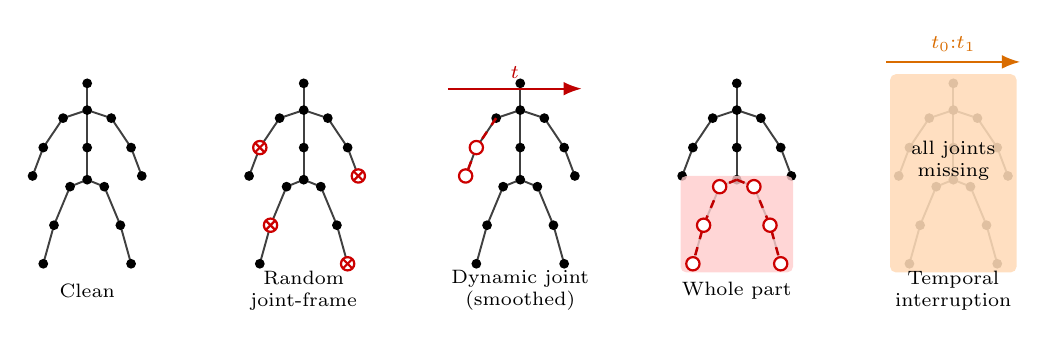
\begin{tikzpicture}[
    font=\scriptsize,
    joint/.style={circle, fill=black, inner sep=1.25pt},
    miss/.style={circle, draw=red!80!black, fill=white, thick, inner sep=1.7pt},
    limb/.style={line width=0.7pt, draw=black!75},
    hidden/.style={line width=0.9pt, draw=red!75!black, dashed},
    label/.style={align=center, font=\scriptsize}
]

\newcommand{\drawskeleton}{
    \coordinate (head) at (0,2.55);
    \coordinate (neck) at (0,2.05);
    \coordinate (spine) at (0,1.35);
    \coordinate (pelvis) at (0,0.75);
    \coordinate (lsho) at (-0.45,1.9);
    \coordinate (lelb) at (-0.82,1.35);
    \coordinate (lhand) at (-1.02,0.82);
    \coordinate (rsho) at (0.45,1.9);
    \coordinate (relb) at (0.82,1.35);
    \coordinate (rhand) at (1.02,0.82);
    \coordinate (lhip) at (-0.32,0.62);
    \coordinate (lknee) at (-0.62,-0.1);
    \coordinate (lfoot) at (-0.82,-0.82);
    \coordinate (rhip) at (0.32,0.62);
    \coordinate (rknee) at (0.62,-0.1);
    \coordinate (rfoot) at (0.82,-0.82);
    \draw[limb] (head)--(neck)--(spine)--(pelvis);
    \draw[limb] (neck)--(lsho)--(lelb)--(lhand);
    \draw[limb] (neck)--(rsho)--(relb)--(rhand);
    \draw[limb] (pelvis)--(lhip)--(lknee)--(lfoot);
    \draw[limb] (pelvis)--(rhip)--(rknee)--(rfoot);
    \foreach \p in {head,neck,spine,pelvis,lsho,lelb,lhand,rsho,relb,rhand,lhip,lknee,lfoot,rhip,rknee,rfoot}
        \node[joint] at (\p) {};
}

\begin{scope}[shift={(0,0)}, scale=0.68]
    \drawskeleton
\end{scope}
\node[label] at (0,-0.9) {Clean};

\begin{scope}[shift={(2.75,0)}, scale=0.68]
    \drawskeleton
    \foreach \p in {lelb,rhand,lknee,rfoot} {
        \node[miss] at (\p) {};
        \draw[red!80!black, thick] ($(\p)+(-0.09,-0.09)$) -- ($(\p)+(0.09,0.09)$);
        \draw[red!80!black, thick] ($(\p)+(-0.09,0.09)$) -- ($(\p)+(0.09,-0.09)$);
    }
\end{scope}
\node[label] at (2.75,-0.9) {Random\\joint-frame};

\begin{scope}[shift={(5.5,0)}, scale=0.68]
    \drawskeleton
    \draw[hidden] (lsho)--(lelb)--(lhand);
    \foreach \p in {lelb,lhand} {
        \node[miss] at (\p) {};
    }
    \draw[-Latex, red!75!black, thick] (-1.35,2.45) -- (1.15,2.45)
        node[midway, above, font=\scriptsize] {$t$};
\end{scope}
\node[label] at (5.5,-0.9) {Dynamic joint\\(smoothed)};

\begin{scope}[shift={(8.25,0)}, scale=0.68]
    \drawskeleton
    \fill[red!20, opacity=0.8, rounded corners=2pt] (-1.05,-0.98) rectangle (1.05,0.82);
    \draw[hidden] (pelvis)--(lhip)--(lknee)--(lfoot);
    \draw[hidden] (pelvis)--(rhip)--(rknee)--(rfoot);
    \foreach \p in {lhip,lknee,lfoot,rhip,rknee,rfoot} {
        \node[miss] at (\p) {};
    }
\end{scope}
\node[label] at (8.25,-0.9) {Whole part};

\begin{scope}[shift={(11,0)}, scale=0.68]
    \drawskeleton
    \fill[orange!28, opacity=0.88, rounded corners=2pt] (-1.18,-0.98) rectangle (1.18,2.72);
    \node[align=center, font=\scriptsize] at (0,1.1) {all joints\\missing};
    \draw[-Latex, orange!85!black, thick] (-1.25,2.95) -- (1.25,2.95)
        node[midway, above, font=\scriptsize] {$t_0{:}t_1$};
\end{scope}
\node[label] at (11,-0.9) {Temporal\\interruption};

\end{tikzpicture}
}
\caption{Conceptual corruption families. Red marks unavailable joints or body
regions; orange marks a contiguous interval in which the complete pose is
unavailable. Random joint-frame masks vary independently, whereas dynamic-joint
masks are temporally smoothed.}
\label{fig:corruptions}
\end{figure}

\begin{figure}[t]
\centering
\resizebox{\textwidth}{!}{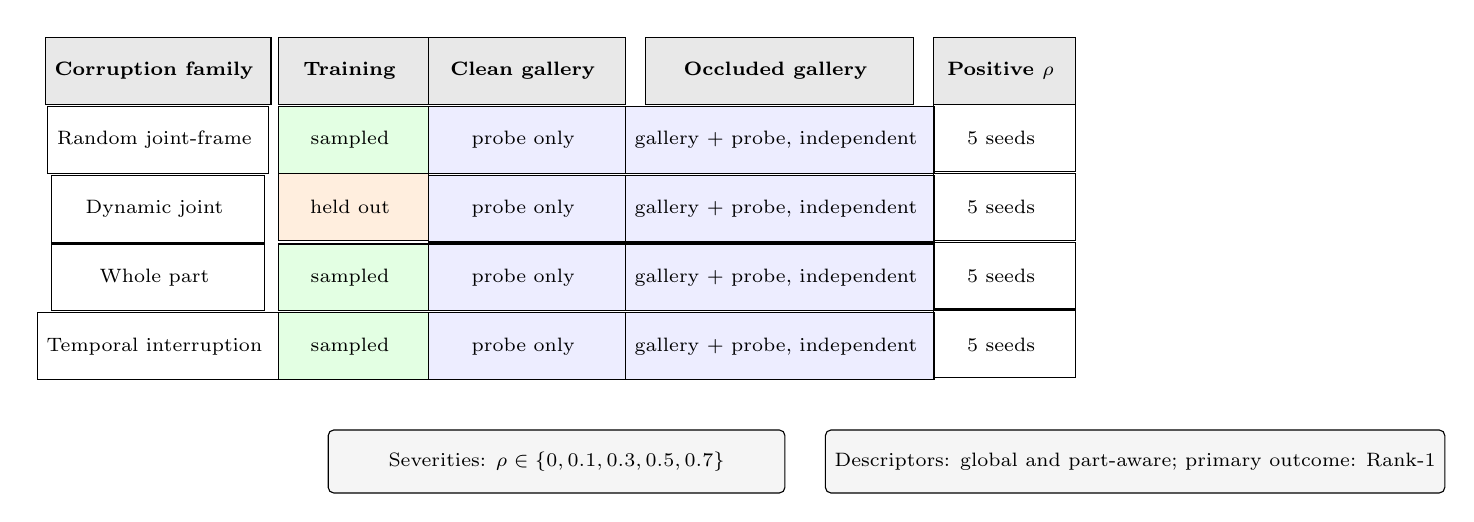
\begin{tikzpicture}[
    font=\scriptsize,
    family/.style={draw, minimum width=27mm, minimum height=8.5mm, align=center},
    train/.style={draw, minimum width=19mm, minimum height=8.5mm, align=center},
    clean/.style={draw, minimum width=25mm, minimum height=8.5mm, align=center},
    occ/.style={draw, minimum width=34mm, minimum height=8.5mm, align=center},
    reps/.style={draw, minimum width=18mm, minimum height=8.5mm, align=center},
    head/.style={fill=gray!18, font=\scriptsize\bfseries},
    yes/.style={fill=green!11},
    held/.style={fill=orange!13},
    protocol/.style={fill=blue!7}
]

\matrix (m) [matrix of nodes, row sep=-\pgflinewidth, column sep=-\pgflinewidth] {
    |[family,head]| Corruption family & |[train,head]| Training &
    |[clean,head]| Clean gallery & |[occ,head]| Occluded gallery &
    |[reps,head]| Positive $\rho$ \\
    |[family]| Random joint-frame & |[train,yes]| sampled &
    |[clean,protocol]| probe only & |[occ,protocol]| gallery + probe, independent &
    |[reps]| 5 seeds \\
    |[family]| Dynamic joint & |[train,held]| held out &
    |[clean,protocol]| probe only & |[occ,protocol]| gallery + probe, independent &
    |[reps]| 5 seeds \\
    |[family]| Whole part & |[train,yes]| sampled &
    |[clean,protocol]| probe only & |[occ,protocol]| gallery + probe, independent &
    |[reps]| 5 seeds \\
    |[family]| Temporal interruption & |[train,yes]| sampled &
    |[clean,protocol]| probe only & |[occ,protocol]| gallery + probe, independent &
    |[reps]| 5 seeds \\
};

\node[draw, rounded corners=2pt, fill=gray!8, align=center, below=5mm of m,
    minimum width=58mm, minimum height=8mm] (sev)
    {Severities: $\rho\in\{0,0.1,0.3,0.5,0.7\}$};
\node[draw, rounded corners=2pt, fill=gray!8, align=center, right=5mm of sev,
    minimum width=58mm, minimum height=8mm] (out)
    {Descriptors: global and part-aware; primary outcome: Rank-1};

\end{tikzpicture}
}
\caption{Evaluation matrix. Dynamic-joint corruption is deliberately held out
from training. Positive-severity results average five deterministic corruption
realizations, and gallery and probe corruptions are independently seeded in the
occluded-gallery protocol.}
\label{fig:evaluation-matrix}
\end{figure}

The primary measure is Rank-1 retrieval. Rank-5, Rank-10, mean average
precision, equal-error rate, and true-acceptance rates are retained in the
released run artifacts but are secondary to the present diagnosis. Development
tables report the mean and sample standard deviation over three training seeds.
For paired development comparisons, each saved outcome is a per-probe correctness value,
averaged over corruption realizations where applicable. We first average the
selected corruption cells within each probe, compute candidate-minus-baseline
differences within each of 12 identities and three matched seeds, and then
resample seeds and identities hierarchically with replacement for 20,000 draws.
Intervals are percentile 95\% intervals. They are used to express uncertainty,
not to support a confirmatory significance claim across the many exploratory
endpoints.

Official-test tables report mean and sample standard deviation over five
matched training seeds. For the standard single-view aggregate, only seed-level
paired outcomes are retained, so candidate-minus-global uncertainty is a paired
$t$ interval over the five seed differences. For pooled multi-view and
synthetic-corruption endpoints, saved per-probe outcomes support a crossed
bootstrap: five seeds and 50 test identities are independently resampled with
replacement for 100,000 draws while preserving candidate--baseline pairing.
Synthetic endpoints first average the four positive severities and four
corruption families within each probe.

\section{Results}

\begin{table}[!t]
\centering
\caption{CASIA-B validation Rank-1 (\%). Clean is mean $\pm$ seed standard
deviation. ``All $>0$'' averages four corruption families at severities 0.1,
0.3, 0.5, and 0.7. Occluded gallery averages the same positive-severity grid.
Single-view averages NM, BG, and CL. Every cell uses three training seeds.}
\label{tab:factorial-results}
\small
\setlength{\tabcolsep}{4pt}
\begin{tabularx}{\textwidth}{@{}>{\raggedright\arraybackslash}Xccccc@{}}
\toprule
\multicolumn{6}{@{}l}{\emph{Global descriptor}} \\
Training objective & Clean & \shortstack{Clean gallery\\all $>0$} &
\shortstack{Clean gallery\\$\rho=0.5$} & \shortstack{Occluded gallery\\all $>0$} &
Single-view \\
\midrule
Metric baseline & 81.52 $\pm$ 2.43 & 63.90 & 64.25 & 67.93 & 67.36 \\
Global SupCon & 79.63 $\pm$ 3.23 & 63.23 & 64.15 & 67.42 & 66.18 \\
Part SupCon & 78.79 $\pm$ 1.14 & 57.78 & 55.57 & 64.26 & 65.33 \\
Part triplet & 81.27 $\pm$ 3.41 & 60.65 & 59.10 & 66.71 & 67.82 \\
Global + part SupCon & 80.05 $\pm$ 1.34 & 60.70 & 59.06 & 65.56 & 65.75 \\
Global + part SupCon (ungated) & 80.89 $\pm$ 1.59 & 61.72 & 60.59 & 66.99 & 66.29 \\
\bottomrule
\end{tabularx}
\vspace{0.5em}

\begin{tabularx}{\textwidth}{@{}>{\raggedright\arraybackslash}Xccccc@{}}
\toprule
\multicolumn{6}{@{}l}{\emph{Reliable-parts descriptor}} \\
Training objective & Clean & \shortstack{Clean gallery\\all $>0$} &
\shortstack{Clean gallery\\$\rho=0.5$} & \shortstack{Occluded gallery\\all $>0$} &
Single-view \\
\midrule
Metric baseline & 83.04 $\pm$ 1.31 & 66.31 & 67.97 & 70.57 & 69.34 \\
Global SupCon & 82.79 $\pm$ 3.36 & 66.21 & 67.85 & 70.38 & 68.66 \\
Part SupCon & 75.42 $\pm$ 2.25 & 54.66 & 52.65 & 61.62 & 61.81 \\
Part triplet & 81.31 $\pm$ 3.42 & 60.66 & 59.11 & 66.73 & 67.82 \\
Global + part SupCon & 77.86 $\pm$ 4.45 & 57.48 & 54.84 & 63.18 & 63.40 \\
Global + part SupCon (ungated) & 78.20 $\pm$ 0.07 & 59.35 & 58.11 & 64.85 & 65.60 \\
\bottomrule
\end{tabularx}
\end{table}

\subsection{Global contrast is neutral; part contrast is harmful}

Table~\ref{tab:factorial-results} shows the complete factorial. With global
matching, the metric baseline attains 81.52\% clean Rank-1, 63.90\% averaged
positive-severity clean-gallery Rank-1, and 67.93\% when both gallery and probe
are corrupted. Global SupCon produces 79.63\%, 63.23\%, and 67.42\%,
respectively. The paired intervals in Table~\ref{tab:paired-results} include
zero for all four global-descriptor endpoints, so this experiment neither
demonstrates a benefit nor a clear robustness penalty from the global SupCon
term.

Part SupCon behaves differently. Its global descriptor loses 6.12 percentage
points on the positive-severity clean-gallery aggregate, with interval
$[-9.54,-2.68]$, and 8.68 points at severity 0.5, with interval
$[-14.50,-3.49]$. The reliable-parts descriptor loses still more. Thus the
failure is not limited to a poorly chosen local matching weight: the shared
global representation also deteriorates when the local contrastive objective is
added.

\begin{table}[!t]
\centering
\caption{Paired Rank-1 difference from the metric baseline in percentage points
(hierarchical 95\% bootstrap interval over seed and validation identity).
Negative values favor the baseline.}
\label{tab:paired-results}
\small
\setlength{\tabcolsep}{4pt}
\begin{tabularx}{\textwidth}{@{}>{\raggedright\arraybackslash}Xlcc@{}}
\toprule
Training objective & Descriptor & Clean & \shortstack{Clean gallery,\\all $>0$} \\
\midrule
Global SupCon & Global & -1.89 [-4.59, +0.46] & -0.67 [-4.21, +3.35] \\
Part SupCon & Global & -2.74 [-6.02, +0.51] & -6.12 [-9.54, -2.68] \\
Part triplet & Global & -0.25 [-4.42, +3.54] & -3.26 [-6.57, +0.21] \\
Global + part SupCon & Global & -1.47 [-4.76, +1.98] & -3.21 [-8.08, +2.40] \\
Global + part (ungated) & Global & -0.63 [-4.63, +4.42] & -2.19 [-4.68, +0.41] \\
Global SupCon & Reliable-parts & -0.25 [-3.11, +2.36] & -0.10 [-2.60, +2.61] \\
Part SupCon & Reliable-parts & -7.62 [-10.86, -4.00] & -11.65 [-15.58, -8.03] \\
Part triplet & Reliable-parts & -1.73 [-5.94, +1.89] & -5.65 [-8.92, -2.17] \\
Global + part SupCon & Reliable-parts & -5.18 [-9.34, -0.63] & -8.83 [-13.78, -2.67] \\
Global + part (ungated) & Reliable-parts & -4.84 [-7.95, -1.81] & -6.96 [-10.56, -3.72] \\
\bottomrule
\end{tabularx}
\vspace{0.5em}

\begin{tabularx}{\textwidth}{@{}>{\raggedright\arraybackslash}Xlcc@{}}
\toprule
Training objective & Descriptor & \shortstack{Clean gallery,\\$\rho=0.5$} &
\shortstack{Occluded gallery,\\all $>0$} \\
\midrule
Global SupCon & Global & -0.10 [-5.43, +6.03] & -0.51 [-2.58, +1.64] \\
Part SupCon & Global & -8.68 [-14.50, -3.49] & -3.67 [-5.70, -1.65] \\
Part triplet & Global & -5.15 [-9.71, -0.32] & -1.22 [-3.69, +0.99] \\
Global + part SupCon & Global & -5.19 [-12.57, +3.73] & -2.37 [-5.48, +1.02] \\
Global + part (ungated) & Global & -3.65 [-8.04, -0.10] & -0.94 [-2.57, +0.80] \\
Global SupCon & Reliable-parts & -0.12 [-3.46, +3.50] & -0.20 [-1.89, +1.59] \\
Part SupCon & Reliable-parts & -15.32 [-21.20, -10.15] & -8.96 [-11.32, -6.53] \\
Part triplet & Reliable-parts & -8.86 [-14.48, -3.24] & -3.85 [-5.97, -1.92] \\
Global + part SupCon & Reliable-parts & -13.13 [-19.81, -4.69] & -7.39 [-10.83, -3.42] \\
Global + part (ungated) & Reliable-parts & -9.85 [-15.36, -5.26] & -5.73 [-7.61, -3.91] \\
\bottomrule
\end{tabularx}
\end{table}

\subsection{Reliability gating is not the primary cause}

The combined gated objective reaches 60.70\% on the positive-severity global
aggregate. Removing reliability weights increases this to 61.72\%, and raises
the corresponding reliable-parts result from 57.48\% to 59.35\%. The recovery
is directionally consistent but remains below the 63.90\% and 66.31\% metric
baselines. Average part reliability (0.502) and presence rate (0.860) are
essentially identical across methods because they are determined by the shared
input sampler. Gating therefore changes how the same observed evidence weights
the auxiliary loss; it does not explain the entire deficit.

\subsection{Training a part head does not make the local matcher stronger}

The part-triplet control closely preserves clean global accuracy (81.27\%) but
falls to 60.65\% on the positive-severity aggregate and 59.10\% at severity 0.5.
Its reliable-parts and global results are nearly identical. The training
diagnostics in Table~\ref{tab:mechanisms} explain this behavior: final normalized
part variance is approximately $1.7\times10^{-6}$, and a nonzero finite
part--triplet cosine is available in only 9 of 96 scheduled diagnostics. The
other diagnostics have a zero-norm gradient for at least one compared loss;
they are not numerical failures. The trained local heads have effectively
collapsed for this objective.

Part SupCon avoids variance collapse: its final variance is
$3.34\times10^{-3}$. Nevertheless, its gradient is less aligned with the
global triplet objective than the global SupCon gradient is. In the combined
model, the mean part--triplet cosine is 0.203, compared with a global--triplet
cosine of 0.446. These cosines are positive, so the data do not support a claim
of direct gradient opposition. They instead show weaker agreement and leave
open other causes, including excessive local invariance, part-specific identity
ambiguity, or mismatch between the local contrastive task and retrieval.

\begin{table}[t]
\centering
\caption{Training diagnostics averaged over three seeds. Part variance is the
mean coordinate-wise variance over the final 20 epochs. Cosines are measured
every five epochs; parentheses give nonzero finite cosine measurements out of
96 scheduled.}
\label{tab:mechanisms}
\small
\setlength{\tabcolsep}{4pt}
\begin{tabular}{@{}lrrr@{}}
\toprule
Objective & Variance ($\times10^{-3}$) & Part--global & Part--triplet \\
\midrule
Metric baseline & 1.269 & -- & -- \\
Global SupCon & 1.300 & -- & -- \\
Part SupCon & 3.338 & -- & 0.212 (95) \\
Part triplet & 0.002 & -- & 0.012 (9) \\
Global + part SupCon & 3.349 & 0.265 (96) & 0.203 (96) \\
Global + part SupCon (ungated) & 3.242 & 0.241 (96) & 0.195 (96) \\
\bottomrule
\end{tabular}
\end{table}

\subsection{Raw part matching resolves the random-head confound}

\begin{table}[!t]
\centering
\caption{Checkpoint-only descriptor controls on CASIA-B validation Rank-1
(\%). All conditions use the same three selected metric-baseline backbones and
the fixed 0.5 fusion weight. ``Fresh random heads'' is the mean across ten
projection seeds; brackets give the range after averaging the three backbone
seeds. No control retrains the backbone or local head.}
\label{tab:descriptor-controls}
\small
\setlength{\tabcolsep}{3.5pt}
\resizebox{\textwidth}{!}{%
\begin{tabular}{@{}lcccc@{}}
\toprule
Descriptor & Clean & \shortstack{Clean gallery\\all $>0$} &
\shortstack{Clean gallery\\$\rho=0.5$} &
\shortstack{Occluded gallery\\all $>0$} \\
\midrule
Global only & 81.52 & 63.90 & 64.25 & 67.93 \\
Saved frozen head & 83.04 & 66.31 & 67.97 & 70.57 \\
Fresh random heads & 83.75 [83.21, 84.26] & 66.50 [66.32, 66.73] &
68.07 [67.71, 68.40] & 70.70 [70.58, 70.81] \\
Raw parts, uniform & 84.43 & 68.11 & 69.99 & 71.71 \\
Raw parts, reliability weighted & \textbf{84.47} & \textbf{68.23} &
\textbf{70.31} & \textbf{71.76} \\
\bottomrule
\end{tabular}%
}
\end{table}

Table~\ref{tab:descriptor-controls} removes the learned projection from the
same checkpoints. Reliability-weighted raw parts improve clean Rank-1 by 2.95
points over global matching, with hierarchical paired interval
$[1.47,4.67]$, and improve the positive-severity aggregate by 4.32 points,
$[3.25,5.35]$. The gain grows to 6.06 points at severity 0.5,
$[4.12,8.29]$, and remains 3.83 points with independently corrupted galleries,
$[3.07,4.72]$. Every training seed improves on both clean and corrupted-probe
endpoints, and the four family-specific corrupted aggregates all increase.

All ten fresh random-head seeds also pass the clean and robustness thresholds:
their clean gains range from 1.68 to 2.74 points and their corrupted-probe gains
from 2.42 to 2.82 points. Thus the original improvement did not depend on one
favorable initialization. However, removing the nonlinear projection is both
deterministic and stronger. The effect is also insensitive to moderate fusion:
raw reliable parts improve the corrupted aggregate by 2.30, 4.32, and 5.68
points at weights 0.25, 0.5, and 0.75, respectively. We retain 0.5 as the
declared primary weight rather than selecting 0.75 after observing validation.

Reliability weighting is not the main source of the raw-descriptor gain.
Relative to uniform averaging, it changes clean Rank-1 by only $+0.04$ points
and the principal corrupted aggregate by $+0.12$ points. The latter interval,
$[+0.02,+0.22]$, is positive but practically small and arises mainly under
whole-part corruption. The supported mechanism is therefore anatomical pooling
and score-level fusion, not a large general advantage from confidence gating.

\subsection{Official CASIA-B test confirmation}

\begin{table}[H]
\centering
\caption{Five-seed CASIA-B official-test Rank-1 (\%), reported as mean
$\pm$ sample standard deviation. The upper panel follows the standard
single-view-gallery protocol and excludes identical views. The lower panel uses
the separately labeled pooled multi-view gallery; ``synthetic'' averages four
corruption families at severities 0.1, 0.3, 0.5, and 0.7.}
\label{tab:official-test}
\small
\setlength{\tabcolsep}{3.5pt}
\begin{tabular}{@{}lcccc@{}}
\toprule
\multicolumn{5}{@{}l}{\emph{Standard single-view protocol}} \\
Descriptor & NM & BG & CL & Average \\
\midrule
Global only & $67.64\pm2.83$ & $49.50\pm1.92$ & $27.91\pm0.94$ & $48.35\pm1.85$ \\
Raw parts, uniform & $74.02\pm3.04$ & $55.56\pm2.04$ & $32.54\pm1.88$ & $54.04\pm2.21$ \\
Raw parts, reliability weighted & $74.14\pm3.04$ & $55.47\pm2.01$ & $32.52\pm1.81$ & $54.04\pm2.18$ \\
\bottomrule
\end{tabular}
\vspace{0.5em}

\begin{tabular}{@{}lccc@{}}
\toprule
\multicolumn{4}{@{}l}{\emph{Pooled multi-view controlled endpoints}} \\
Descriptor & Uncorrupted & \shortstack{Synthetic,\\clean gallery} &
\shortstack{Synthetic,\\occluded gallery} \\
\midrule
Global only & $68.06\pm0.50$ & $48.90\pm0.63$ & $54.34\pm0.63$ \\
Raw parts, uniform & $74.76\pm0.47$ & $55.13\pm1.22$ & $59.88\pm0.90$ \\
Raw parts, reliability weighted & $74.64\pm0.45$ & $55.29\pm1.22$ & $59.96\pm0.90$ \\
\bottomrule
\end{tabular}
\end{table}

Table~\ref{tab:official-test} answers the fifth study question without changing
the selected objective, descriptor, or fusion weight. On the standard protocol,
reliability-weighted raw parts improve the three-condition average over global
matching by 5.69 percentage points; the paired five-seed 95\% interval is
$[5.19,6.20]$. The condition-specific gains are 6.50 points for NM,
$[6.16,6.84]$; 5.97 for BG, $[5.73,6.22]$; and 4.61 for CL,
$[3.51,5.71]$.

The saved test-identity outcomes permit stronger paired analysis for the pooled
protocol. Reliability-weighted raw parts gain 6.58 points on uncorrupted probes,
with crossed-bootstrap interval $[5.37,7.83]$; 6.39 points over the positive-
severity synthetic grid with a clean gallery, $[5.40,7.40]$; and 5.63 points
with independently corrupted galleries, $[4.89,6.40]$. Uniform and reliability-
weighted raw matching remain practically tied on the standard average: the
reliability-minus-uniform difference is $+0.004$ points with paired interval
$[-0.059,+0.067]$. Reliability gives small positive synthetic-grid differences
of 0.16 points for the clean gallery and 0.08 points for the occluded gallery,
but these do not alter the mechanism conclusion: anatomical score fusion
provides the material gain.

\subsection{Efficiency}

The common backbone contains 1.69 million parameters. Mean training time is
1.63 hours for the metric baseline, 1.89 hours for global SupCon, and
1.97--1.99 hours for the combined or part-triplet variants on the recorded H100
MIG environment. This is approximately 21\% overhead for the combined model,
substantially below an initial twofold estimate. These measurements do
not establish deployment cost: the reliable-parts descriptor stores and scores
five additional local embeddings, so inference latency, gallery storage, and
pairwise scoring throughput must be measured before an efficiency claim is
made.

\section{Discussion}

\subsection{What the factorial establishes}

The controlled comparison rejects the original hypothesis that adding
reliability-gated part SupCon to the selected metric baseline improves
occlusion robustness. The conclusion is stronger than a single unfavorable
mean: the degradation is visible across descriptors and gallery protocols, and
the paired identity-level interval excludes zero for the principal corrupted-
probe aggregate. Global SupCon is comparatively benign but offers no
demonstrated advantage. Ungating helps the combined objective but does not
restore the baseline, while part triplet reveals a separate collapse mode.

The most constructive outcome is the separation between training and matching.
Local pooling plus reliability-weighted scoring can help without an explicit
local objective, whereas the tested local objectives degrade the representation.
The checkpoint-only controls sharpen this suggestion: the best local evidence
is already present before a part head. The raw descriptor changes neither the
backbone nor its training objective, adds no learned parameters, and improves
all four corruption families. Random nonlinear heads preserve part of this
geometry, while the tested supervised heads distort or collapse it.

The official test extends the positive matching result beyond the development
identities, but it does not retest all six training objectives. The negative
conclusion about auxiliary part training therefore remains a controlled
development result; the official confirmation concerns the selected metric
baseline and the three matching descriptors.

\subsection{Official confirmation and remaining evaluation}

The candidate carried into official evaluation is reliability-weighted
normalized raw-part pooling with a 0.5 global--local score mixture. Its gain is
preserved across five new full-training runs and all three standard CASIA-B
conditions. Uniform weighting remains an important ablation because its
performance is nearly identical; we do not claim that reliability is a major
independent contribution. Likewise, the 0.75 mixture is reported only as
development sensitivity and is not promoted after observing validation.

A frozen-backbone head-only study remains useful as a mechanism experiment.
Global-to-part stop-gradient distillation and a low-weight part triplet with an
explicit variance floor can test whether a learned head can retain the raw
geometry. It is no longer a prerequisite for defining the primary method: if
neither head exceeds the fixed raw descriptor without violating clean accuracy
or the $10^{-4}$ variance floor, the raw descriptor remains the confirmatory
candidate. The official CASIA-B test has now been consumed and should not guide
further tuning. The next priorities are real occlusion, an established external
backbone, and another dataset rather than another broad loss-weight sweep.

\section{Limitations and Validity Threats}

\paragraph{Single-dataset official confirmation.}
The study reports the official CASIA-B test identities for the selected metric
baseline and matching descriptors, but not for all six development objectives
or reproduced state-of-the-art systems. The official experiment confirms
within-dataset transfer of the matching decision; it is not by itself evidence
of cross-dataset generalization or a leaderboard claim.

\paragraph{Synthetic rather than real occlusion.}
The corruptions are controlled missingness mechanisms. They do not reproduce
left/right swaps, cross-person joint assignment, smooth but anatomically wrong
tracks, or population and camera shifts. At least one real-occlusion endpoint
is necessary before claiming operational robustness.

\paragraph{One pose source and one backbone.}
All runs use the same HRNet-derived 2D pose and an internal multistream graph
network. A general claim that part supervision is harmful requires replication
with another pose source, dataset, and established backbone. Conversely, a
positive redesigned method must outperform reproduced external baselines rather
than only this internal control.

\paragraph{Three development seeds and five confirmation seeds.}
Three seeds support the factorial diagnosis but provide limited precision for
model-training variability. The official comparison uses five matched seeds;
its paired standard-protocol interval still has only four degrees of freedom.
Identity resampling in the pooled-outcome bootstrap represents test-population
variation but does not create additional independent model trainings. No
family-wise error claim is made over the many exploratory corruptions and
descriptors.

\paragraph{Descriptor development on the same validation identities.}
The raw descriptor, uniform/reliability ablation, random-head controls, and
fusion sensitivity are all evaluated on the same 12 development identities.
The primary 0.5 fusion weight and acceptance thresholds were declared before
running these controls, but choosing the raw descriptor still constitutes model
development. The higher validation score at weight 0.75 must not be treated as
confirmatory. The fixed 0.5 candidate has now been evaluated on the official
test; those outcomes must not be used for another tuning round. External
datasets remain required.
Gradient cosines are computed at the shared paired-view feature tensor;
clean-anchor CE occupies a different batch slice and is therefore orthogonal by
construction at that tensor. We consequently do not interpret clean-CE cosine
values. Parameter-level diagnostics are needed for any new joint training.

\paragraph{Reproducibility provenance.}
The factorial records source SHA-256 ``ad96b902\ldots'' and the descriptor
controls record ``eddf23a2\ldots''; both use dataset SHA-256
``123e838c\ldots''. The official confirmation records source SHA-256
``7a351cac\ldots'', dataset SHA-256 ``9823d021\ldots'', and configuration
fingerprint ``f25bd174\ldots''. Every condition retains its configuration,
environment, selected epoch, aggregate metrics, and probe outcomes. The five
official runs used two H100 NVL MIG profiles but identical software, source,
data, and configuration hashes. However, the runs record
``not-a-git-checkout''.
The release should initialize a canonical repository, tag the exact source
snapshot, lock dependencies, and provide a manifest connecting every reported
cell to its run directory.

\section{Ethical Considerations}

Gait is biometric information and can enable remote identification without an
individual's awareness. Improvements in occlusion handling do not remove the
requirements for lawful purpose, consent where applicable, access control,
retention limits, and human oversight. Evaluation should include demographic
and disability-related audits, including mobility aids and atypical gait. The
present CASIA-B data cannot support fairness or deployment claims, and the
reported synthetic robustness should not be interpreted as operational
reliability.

\section{Conclusion}

In a controlled six-objective, three-seed study, the tested part-level
supervised contrastive objective does not improve occlusion-robust pose gait
recognition. It substantially reduces robustness relative to a shared
classification-plus-triplet baseline. Reliability gating is not the sole
cause, global SupCon is inconclusive, and part-triplet training collapses the
local embeddings. Checkpoint-only controls resolve the apparent random-head
confound: normalized raw part pools improve clean Rank-1 by 2.95 points and the
principal corrupted-probe aggregate by 4.32 points at the declared 0.5 fusion
weight, with paired intervals excluding zero. Ten fresh random projections also
help, but less. Uniform and reliability-weighted raw matching are nearly tied,
so anatomical pooling and score fusion---not strong evidence for confidence
gating---form the supported mechanism. The justified candidate is therefore a
globally trained backbone with parameter-free raw part matching. Five-seed
official-test evaluation confirms this candidate: under the standard
single-view protocol, reliability-weighted raw parts raise the three-condition
average from $48.35\pm1.85$\% to $54.04\pm2.18$\%, a paired gain of 5.69 points
with interval $[5.19,6.20]$. Pooled uncorrupted and synthetic test endpoints
show gains of 5.63--6.58 points. Uniform raw matching remains effectively tied,
reinforcing that anatomical fusion rather than reliability weighting supplies
the material benefit. Real occlusion, an external backbone, and additional
datasets remain necessary before a broad robustness claim is warranted.

\begin{thebibliography}{25}

\bibitem{chen2020simclr}
Chen, T., Kornblith, S., Norouzi, M., Hinton, G.:
A simple framework for contrastive learning of visual representations.
In: Proceedings of ICML. pp. 1597--1607 (2020)

\bibitem{he2020moco}
He, K., Fan, H., Wu, Y., Xie, S., Girshick, R.:
Momentum contrast for unsupervised visual representation learning.
In: Proceedings of CVPR. pp. 9729--9738 (2020)

\bibitem{khosla2020supervised}
Khosla, P., et al.:
Supervised contrastive learning.
In: Advances in Neural Information Processing Systems, vol. 33,
pp. 18661--18673 (2020)

\bibitem{yan2018stgcn}
Yan, S., Xiong, Y., Lin, D.:
Spatial temporal graph convolutional networks for skeleton-based action
recognition. In: Proceedings of AAAI, vol. 32 (2018)

\bibitem{thoker2021skeleton}
Thoker, F.M., Doughty, H., Snoek, C.G.M.:
Skeleton-contrastive 3D action representation learning.
In: Proceedings of ACM Multimedia. pp. 1655--1663 (2021)

\bibitem{teepe2021gaitgraph}
Teepe, T., Khan, A., Gilg, J., Herzog, F., H\"ormann, S., Rigoll, G.:
GaitGraph: Graph convolutional network for skeleton-based gait recognition.
In: Proceedings of ICIP. pp. 2314--2318 (2021)

\bibitem{fan2022opengait}
Fan, C., Liang, J., Shen, C., Hou, S., Huang, Y., Yu, S.:
OpenGait: Revisiting gait recognition toward better practicality.
In: Proceedings of CVPR. pp. 9707--9716 (2023)

\bibitem{li2024survey}
Li, T., et al.:
A survey on gait recognition against occlusion: taxonomy, dataset and
methodology. PeerJ Computer Science 10, e2602 (2024)

\bibitem{huang2024occluded}
Huang, P., et al.:
Occluded gait recognition with mixture of experts: an action detection
perspective. In: Proceedings of ECCV. pp. 380--397 (2024)

\bibitem{chen2023iopstl}
Chen, Y., et al.:
Exploring self-supervised skeleton-based action recognition in occluded
environments. arXiv:2309.12029 (2023)

\bibitem{rao2024skeleton}
Rao, H., Miao, C.:
Skeleton prototype contrastive learning with multi-level graph relation
modeling for unsupervised person re-identification.
In: QSHINE. pp. 306--321. Springer (2024)

\bibitem{liao2020posegait}
Liao, R., Yu, S., An, W., Huang, Y.:
A model-based gait recognition method with body pose and human prior knowledge.
Pattern Recognition 98, 107069 (2020)

\bibitem{teepe2022gaitgraph2}
Teepe, T., Gilg, J., Herzog, F., H\"ormann, S., Rigoll, G.:
Towards a deeper understanding of skeleton-based gait recognition.
In: Proceedings of the CVPR Workshops. pp. 1569--1577 (2022)

\bibitem{fu2023gpgait}
Fu, Y., Meng, S., Hou, S., Hu, X., Huang, Y.:
GPGait: Generalized pose-based gait recognition.
In: Proceedings of ICCV. pp. 19595--19604 (2023)

\bibitem{fan2024skeletongait}
Fan, C., Ma, J., Jin, D., Shen, C., Yu, S.:
SkeletonGait: Gait recognition using skeleton maps.
In: Proceedings of AAAI, vol. 38(2), pp. 1662--1669 (2024)

\bibitem{fan2020gaitpart}
Fan, C., Peng, Y., Cao, C., Liu, X., Hou, S., Chi, J., Huang, Y., Li, Q., He, Z.:
GaitPart: Temporal part-based model for gait recognition.
In: Proceedings of CVPR. pp. 14225--14233 (2020)

\bibitem{lin2021gaitgl}
Lin, B., Zhang, S., Yu, X.:
Gait recognition via effective global-local feature representation and local
temporal aggregation. In: Proceedings of ICCV. pp. 14648--14656 (2021)

\bibitem{huang2021local}
Huang, Z., Xue, D., Shen, X., Tian, X., Li, H., Huang, J., Hua, X.-S.:
3D local convolutional neural networks for gait recognition.
In: Proceedings of ICCV. pp. 14920--14929 (2021)

\bibitem{yu2006casia}
Yu, S., Tan, D., Tan, T.:
A framework for evaluating the effect of view angle, clothing and carrying
condition on gait recognition. In: Proceedings of ICPR. pp. 441--444 (2006)

\bibitem{sun2019hrnet}
Sun, K., Xiao, B., Liu, D., Wang, J.:
Deep high-resolution representation learning for human pose estimation.
In: Proceedings of CVPR. pp. 5693--5703 (2019)

\bibitem{lin2014coco}
Lin, T.-Y., et al.:
Microsoft COCO: Common objects in context.
In: Proceedings of ECCV. pp. 740--755 (2014)

\bibitem{hermans2017triplet}
Hermans, A., Beyer, L., Leibe, B.:
In defense of the triplet loss for person re-identification.
arXiv:1703.07737 (2017)

\bibitem{zhu2021grew}
Zhu, Z., Guo, X., Yang, T., Huang, J., Deng, J., Huang, G., Du, D., Lu, J.,
Zhou, J.:
Gait recognition in the wild: A benchmark.
In: Proceedings of ICCV. pp. 14789--14799 (2021)

\bibitem{zheng2022gait3d}
Zheng, J., Liu, X., Liu, W., He, L., Yan, C., Mei, T.:
Gait recognition in the wild with dense 3D representations and a benchmark.
In: Proceedings of CVPR. pp. 20228--20237 (2022)

\bibitem{cosma2026gaitpt}
Cosma, A., Catruna, A.E., Radoi, E.:
On model and data scaling for skeleton-based self-supervised gait recognition.
In: Proceedings of AAAI, vol. 40(5), pp. 3434--3442 (2026)

\end{thebibliography}

\end{document}
